\section{\acrshort{wdias} Database Structure}
\label{se:db_struct}

The foundation of the \acrshort{wdias} is data-centric. To understand the underline design decisions of the \acrshort{wdias} database structure, it needs to deeply look into the weather data timeseries.
\paragraph{Timeseries}-- \emph{A timeseries is simply a series of data points ordered in time}. In the weather domain, its interest in timeseries in perspective of observations to forecasting. Each timeseries, the data points can be formed in different formats as well. For example, scalar (0D), vector (1D), grid (2D), and polygon (2D).

As per the above interpretation, a timeseries have data points ordered in time. Other than that, timeseries have other information which is known as \emph{timeseries metadata} which can use to uniquely identify one timeseries from another. As an example, a weather station can be placed on a location and it can keep measure variables which are called \emph{parameters} such as temperature, precipitation and wind direction which can produce different timeseries. Even we can use the location as metadata to identify the timeseries, that is not enough to separately identify the parameters. Thus we need to use a set of attributes to uniquely identify a timeseries. In the next \cref{subse:timeseries_key_attributes}, we describe key attributes which are using by the \acrshort{wdias} to uniquely identify a timeseries.

\dbc{Clearly mention why a hierarchical design is needed.}
\gkc{Added it after the \cref{subse:timeseries_key_attributes}}

%%%%%%%%%%%%%%%%%%%%%%%%%%%%%%%%%%%%%%%%%%%%%%%%%%%%%%%%%%%%%%%%%%%%%%%%%%%%%%%%
\subsection{Key Attributes of Timeseries}
\label{subse:timeseries_key_attributes}
\paragraph{Module ID}-- String field which describe the source of the data generated. e.g., hec-hms, flow2d, weather-station, etc

\paragraph{Value Type}-- Scalar, Vector, Grid are the Value Types that are interested in the \acrshort{wdias}.

\paragraph{Location}-- Location of the timeseries. All locations have a unique String identifier called locationId. Further, two types of location types are interested in the WDIAS, namely:
\begin{itemize}
  \item \emph{Point locations}-- Contains a name that is human readable. lat and lon of the location on the earth surface.
  \begin{lstlisting}[language=Python]
    {
        "locationId": "wdias-hanwella",
        "name": "Hanwella",
        "lat": 6.909722222,
        "lon": 80.08166667
    }
  \end{lstlisting}
  \dbc{Remove additional line.}
  \gkc{This space is adding by itemize. I applied in all the places. Could not find how to remove it. Otherwise, need to remove itemize.}
  \item \emph{Regular Grid locations} -- Contains a name that is human readable. The grid presents by dividing into equal size cells. Thus, it needs the number of rows and columns. 
  And the location of the first cell and the width and height of it.
  \begin{lstlisting}[language=Python]
      {
        "locationId": "wdias_kelani_basin",
        "description": "Kelani Basin",
        "rows": 120,
        "columns": 139,
        "geoDatum": "Kandawala",
        "gridFirstCell": {
            "firstCellCenter": {
                "x": 397074.0,
                "y": 504875.0
            },
            "xCellSize": 250.0,
            "yCellSize": 250.0
        }
    }
  \end{lstlisting}
  \item \emph{Irregular Grid locations} -- (endpoints are available within the WDIAS system, but skipped since it is out of the interest of the scope.)
\end{itemize}

\paragraph{Parameter}
Parameter describes the variable measuring against a location. All parameters have a unique String identifier called \emph{parameterId}. A parameter can be used in multiple locations. While defining a parameter, three required fields need to be provided such as variable, unit and \emph{parameterType}.

\begin{itemize}  
  \item \emph{Variable} -- Nature of the variable measuring. Example Precipitation, Temperature and Water Level etc
  \item \emph{Unit} -- metric unit of measuring
  \item \emph{Parameter Type} -- Should be one of Instantaneous, Accumulative, or Mean
  \begin{lstlisting}[language=Python]
    {
      "parameterId": "O.Precipitation",
      "variable": "Precipitation",
      "unit": "mm",
      "parameterType": "Instantaneous"
    }
  \end{lstlisting}
\end{itemize}

\subsubsection{Timeseries Type}
Timeseries Type can be redefined with the system setup. \acrshort{wdias} defined the following types for during the setup. Timeseries type can be a combination of a source followed by category:
\begin{itemize}
  \item Sources - External or simulated. \emph{External} means whether timeseries is taken from an external source, and \emph{simulated} means it generated by simulations of the users.
  \item Category - Historical or forecast. \emph{Historical} means whether timeseries have continuous data such as observations from a weather station. \emph{forecast} means discrete set of timeseries data produce by forecasting.
\end{itemize}
\dbc{Explain each with sufficient detail.}
\gkc{FIXED}

\paragraph{Time Step}-- All TimeSteps has a unique String identifier called timeStepId. Unit should be one of Second, Minute, Hour, Day, Week, Month, Year, or NonEqualDistance. One of multiplier or divider can be used to define the interval between each measurement.
\begin{lstlisting}[language=Python]
{
    "timeStepId": "each_min",
    "unit": "Minute",
    "multiplier": 1,
    "divider": 0
}
\end{lstlisting}

Among the above key attributes; Location, Parameter and Time Step attributes are composite attributes. But each of them has a unique identifier.
Given that, a timeseries can uniquely identify by moduleId, valueType, parameterId, locationId, timeseriesType and timeStepId.
\begin{lstlisting}[language=Python]
{
	"moduleId": "HEC-HMS",
	"valueType": "Scalar",
	"parameterId": "O.Precipitation",
	"locationId": "wdias_hanwella",
	"timeseriesType": "External_Historical",
	"timeStepId": "each_hour",
}
\end{lstlisting}

%%%%%%%%%%%%%%%%%%%%%%%%%%%%%%%%%%%%%%%%%%%%%%%%%%%%%%%%%%%%%%%%%%%%%%%%%%%%%%%%
Even a timeseries consists of data points, the data for each data point can vary based on the valueType. Scalar data point only consist of a single value. And Vector data point consists of two values such as magnitude and the direction of the Vector. But for Grid data, a point can consist of multiple values. To get the advantage of storing data efficiently, we can use a set of different databases based on the advantage of using them for each valueType. Other than the valueType attribute, other attribute does not much impact on the data size.

Further, it is will be difficult to search for the timeseries data, if those are stored over multiple data sources, and difficult to avoid having duplicates. Thus it adds low overhead to have a single data source to look into while searching for the timeseries metadata. The load on the above data source can reduce by using a caching mechanism. To support search queries with lower latency, it required to use indexing for the fast search for timeseries metadata. Further, Geo-based indexing is required to support Geo-based search queries based on the locations. 

Considering the above facts, we can not achieve all of the benefits using one of the database systems available. Thus it required to have a database structure that is capable of proving all of the above capabilities via combining. According to the design principle of microservices architecture, we created microservice for each of the valueType with following the concept of Database per Service as described in the \emph{Database per Service} in \cref{subse:database_per_service}. In \cref{sebse:wdias_microservices} those microservices are group as \emph{adapters} that share an \acrshort{api} to interact with while keeping the persistent data private.

\begin{figure}[htp]
    \centering
    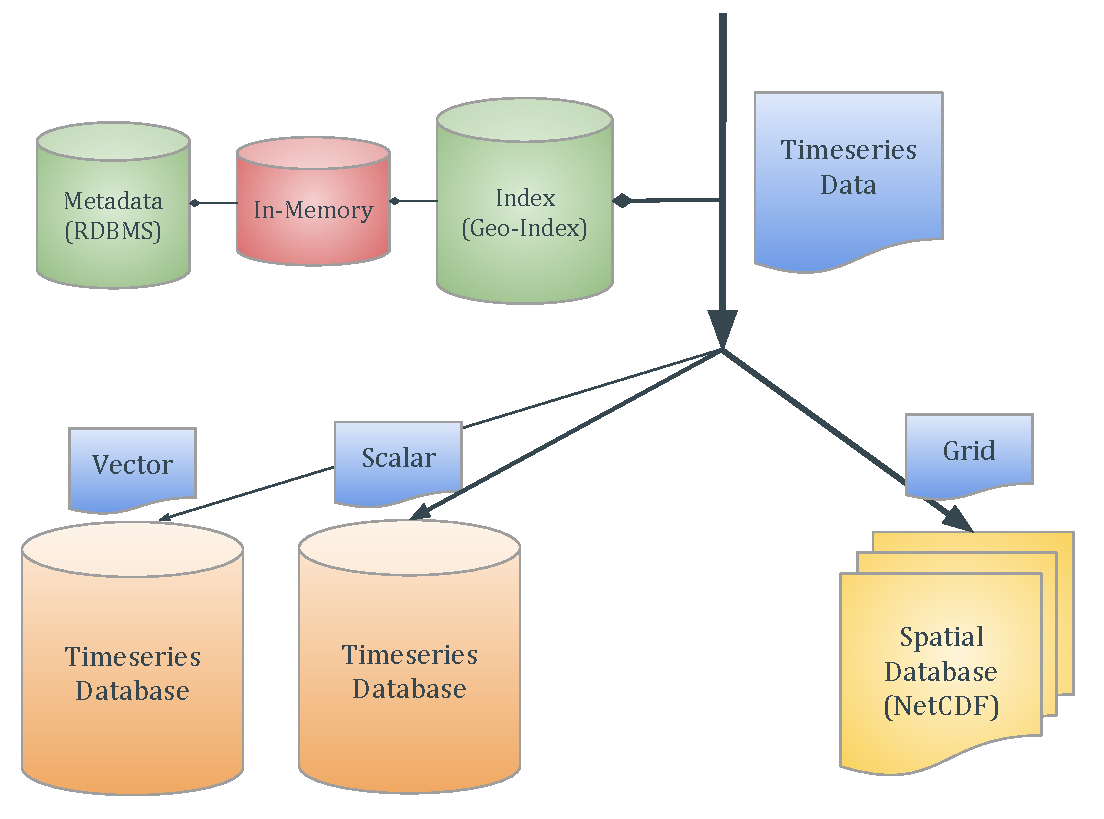
\includegraphics[width=0.8\textwidth]{method/microservice/wdias_database_structure.pdf}
    \caption{\acrshort{wdias} database structure}
    \label{fi:database_structure}
\end{figure}

\dbc{Fig. 3.6 needs a more meaningful title.}
\gkc{Updated. I think hierarchical database does not make sense in this case. May be that's why you asked for change few time, sir.}

\cref{fi:database_structure} shows the \acrshort{wdias} database structure.
The following sections describe the database structure of \acrshort{wdias} with compare to the design with more details on how is support the microservice architecture.

%%%%%%%%%%%%%%%%%%%%%%%%%%%%%%%%%%%%%%%%%%%%%%%%%%%%%%%%%%%%%%%%%%%%%%%%%%%%%%%%
\subsection{Timeseries Metadata Storage}
\label{subse:mysql}
\dbc{Needs a more meaningful Sec. title}
\gkc{UPDATED}

As described in the above section, to reduce the overhead while searching for timeseries and handling duplicates, it required to have a timeseries metadata store. Since metadata consists of multiple key attributes, the data can be efficiently store using a \acrfull{rdbms}. This helps to store data without any duplicates and store the data with normalization. As an example, the parameter attribute can have one or two dozen of values. Using an \acrshort{rdbms}, those values can be stored once and reuse with defining timeseries against location via reference.

\acrshort{wdias} is using SQL as the \acrfull{rdbms}. 
Since the \acrshort{wdias} scope is to use open source tools, it is using  MySQL as a persistent database for storing timeseries metadata described above.
One instance of  MySQL is using only by adapter-metadata service.
Other than that, another instance of  MySQL is using for adapter-extension which will be described in more detail \cref{se:data_preprocess}.
 MySQL is used only for these services, those will only keep the consistency of the schema for timeseries metadata and extension metadata.
As mentioned in \cref{subse:redis}, it uses  Redis instance is using for caching the data from  MySQL, since the  MySQL database instances, itself not going to get much load.
Other than MySQL, many open source databases can be used to replace the same functionality.
\dbc{First start with a brief discussion on why a RDBMS is needed}
\gkc{ADDED}

%%%%%%%%%%%%%%%%%%%%%%%%%%%%%%%%%%%%%%%%%%%%%%%%%%%%%%%%%%%%%%%%%%%%%%%%%%%%%%%%
\subsection{Timeseries Database}
\label{subse:influxdb}
Among several timeseries open source databases,  InfluxDB \cite{influxdbInfluxDBDocumentation} \hl{is using a unique database indexing algorithm to gain higher performance while storing timeseries data} when compared to other databases available. Also, it has better support, higher usage and has following supports;
\begin{itemize}
  \item Open timeseries DB with MIT license
  \item Support SQL-Like query language
  \item Clustering available with a commercial version
\end{itemize}
Other than  InfluxDB, another database is Elastic Search which is mainly using for indexing for searching.
With changing the configurations of the  InfluxDB, it is possible to adapt as required. As mention in \cite{influxdbInfluxDBDocumentation}, 
 InfluxDB can setup on a computer that will give the required performance. Going further, users can use the commercial version of  InfluxDB to gain more performance.

Two instances of  InfluxDB is using in the WDIAS system by adapter-scalar and adapter-vector services. For the scalability, the system uses \emph{Database per Service} as mentioned in \cref{subse:database_per_service}.
But further, it split into two services, referring to \cref{subse:scale_cube}, the Z-axis scaling, the data is partitioned among a few servers based on valueType key attribute of timeseries.
Which also conclude the concept of splitting into more services based on other key attributes such as timeseriesType, if further performance required.

%%%%%%%%%%%%%%%%%%%%%%%%%%%%%%%%%%%%%%%%%%%%%%%%%%%%%%%%%%%%%%%%%%%%%%%%%%%%%%%%
\subsection{\acrfull{netCDF}}
\label{subse:netcdf}
\acrshort{netCDF} \cite{unidataUnidataNetCDF} is a self-describing, machine-independent data formats that support the creation, access, and sharing of array-oriented scientific data.
And it also has the support for parallel file access.
NetCDF is widely using in the scientific domain due to it has the capability of storing data in multi-dimensions easily and flexibility with storing many of the scientific data. Due to its capability of storing scientific data efficiently, \acrshort{wdias} using it for storing the Grid data.

%%%%%%%%%%%%%%%%%%%%%%%%%%%%%%%%%%%%%%%%%%%%%%%%%%%%%%%%%%%%%%%%%%%%%%%%%%%%%%%%
\subsection{Document-oriented Database}
\label{subse:mongodb}

\acrshort{wdias} is using  MongoDB as the document-oriented database, as it has the Geo searching capabilities.
 MongoDB \cite{mongodbMongoDBManual} is a general-purpose, document-based, distributed database. And it supports:
\dbc{Need for a mix of relational, time series, document stores, and in-memory need to be first mentioned and justified in high-level design of WDIAS above.}
\gkc{Adding those details in \cref{se:high_level_design} may confuse the reader. At that point it didn't go through that much of details of the wdias. I added some justification at the end of \cref{subse:timeseries_key_attributes}. Let me know if we want to highlight it with a different section there.}
\begin{itemize}
  \item Supports query operations on geospatial data \cite{mongodbMongoDBManual}
  \item Clustering and Sharding available for scalability and reliability
\end{itemize}
 MongoDB geospatial features are using to support Geo queries in the WDIAS. Other than that, external timeseries metadata queries are served by the indexed timeseries metadata data.
If metadata not present in the adapter-query if fetch data from the adapter-metadata, then indexed and cache in the  MongoDB. Vise a versa, if new timeseries create in the adapter-metadata, it triggers an event to adapter-query to index the new timeseries.
In \cref{subse:scale_cube}, the Y-axis scaling concept is using here by splitting into the multiple services based on the functionality and scale of the system.

%%%%%%%%%%%%%%%%%%%%%%%%%%%%%%%%%%%%%%%%%%%%%%%%%%%%%%%%%%%%%%%%%%%%%%%%%%%%%%%%
\subsection{In-Memory Database}
\label{subse:redis}
\acrshort{wdias} is using  Redis \cite{redisRedisDocumentation} as the In-Memory database, since it is a widely used tool with good support, and it supports few other features such as Publisher Subscriber capabilities.
 Redis is an open-source (BSD licensed), used as a database, cache. Clustering is available for scalability.
 Redis uses as in-memory caching for fast access the frequent access data in adapter-metadata and adapter-extension.
Other than that, adapter-status uses  Redis as a key-value pair store for getting the status for async handling requests such as storing Grid data.
In adapter-extension uses Redis's Publisher Subscriber capabilities to create a cronjob in extension-scheduler when a new extension creates on \cref{se:data_preprocess}
